% answers.tex —— 2004 年·春季上海卷 · 参考答案与详细解析片段
% 由 tools/generate_projects.py 依来源总账自 2004/2004_数学真题_春季上海_试题.md + 2004/2004_数学真题_春季上海_解析正文.md + 2004/2004_数学真题_春季上海_答案要点.md 生成，勿手改（改源 MD 后重跑）


\begin{gktip}
以下推导基于本项目的逐题题面转录，属于独立生成内容而非官方答案。来源没有答案页。第 18 题的 $x/p$ 记号冲突原样保留并分别讨论，不以推测修订代替原文。
\end{gktip}

\begin{answer}
\gksolhead{1}{}

\textbf{题目}：

若复数 $z$ 满足 $z(1+i)=2$，则 $z$ 的实部是 $\underline{\qquad}$。

\Needspace{4\baselineskip}
\textbf{解析}

\nopagebreak[4]
\[z=\frac2{1+i}=1-i,\]

故 $\operatorname{Re}z=1$。

\gkanswer{答案：$1$}

\end{answer}
\begin{answer}
\gksolhead{2}{}

\textbf{题目}：

方程 $\lg x+\lg(x+3)=1$ 的解 $x=\underline{\qquad}$。

\Needspace{4\baselineskip}
\textbf{解析}

\Needspace{5\baselineskip}
定义域要求 $x>0$。由对数运算得

\nopagebreak[4]
\[x(x+3)=10,\]

即 $(x+5)(x-2)=0$。结合定义域，$x=2$。

\gkanswer{答案：$2$}

\end{answer}
\begin{answer}
\gksolhead{3}{}

\textbf{题目}：

在 $\triangle ABC$ 中，$a,b,c$ 分别是 $\angle A$、$\angle B$、$\angle C$ 所对的边。若 $\angle A=105^\circ$，$\angle B=45^\circ$，$b=2\sqrt{2}$，则 $c=\underline{\qquad}$。

\Needspace{4\baselineskip}
\textbf{解析}

\Needspace{5\baselineskip}
$\angle C=180^\circ-105^\circ-45^\circ=30^\circ$。由正弦定理

\nopagebreak[4]
\[c=b\frac{\sin C}{\sin B}=2\sqrt2\cdot\frac{1/2}{\sqrt2/2}=2.\]

\gkanswer{答案：$2$}

\end{answer}
\begin{answer}
\gksolhead{4}{}

\textbf{题目}：

过抛物线 $y^2=4x$ 的焦点 $F$ 作垂直于 $x$ 轴的直线，交抛物线于 $A$、$B$ 两点，则以 $F$ 为圆心、$AB$ 为直径的圆方程是 $\underline{\qquad}$。

\Needspace{4\baselineskip}
\textbf{解析}

抛物线 $y^2=4x$ 的焦点为 $F(1,0)$。过焦点且垂直于 $x$ 轴的弦端点为 $(1,2)$、$(1,-2)$，故 $AB=4$，以 $AB$ 为直径的圆半径为 $2$，圆心为 $F$。

\gkanswer{答案：$(x-1)^2+y^2=4$}

\end{answer}
\begin{answer}
\gksolhead{5}{}

\textbf{题目}：

已知函数 $f(x)=\log_3\left(\dfrac{4}{x}+2\right)$，则方程 $f^{-1}(x)=4$ 的解 $x=\underline{\qquad}$。

\Needspace{4\baselineskip}
\textbf{解析}

\Needspace{5\baselineskip}
对方程 $f^{-1}(x)=4$ 两边作用 $f$，得 $x=f(4)$。代入函数定义：

\nopagebreak[4]
\[x=f(4)=\log_3\left(\frac44+2\right)=\log_3 3=1.\]

函数值 $f(4)$ 有定义，故方程的解为 $1$。

\gkanswer{答案：$1$}

\end{answer}
\begin{answer}
\gksolhead{6}{}

\textbf{题目}：

如图，在底面边长为 $2$ 的正三棱锥 $V-ABC$ 中，$E$ 是 $BC$ 的中点。若 $\triangle VAE$ 的面积是 $\dfrac{1}{4}$，则侧棱 $VA$ 与底面所成角的大小为 $\underline{\qquad}$。（结果用反三角函数值表示。）
\nopagebreak[4]
\begin{center}% Q6：线型按原页复现。空间位置仅作示意，不按比例。
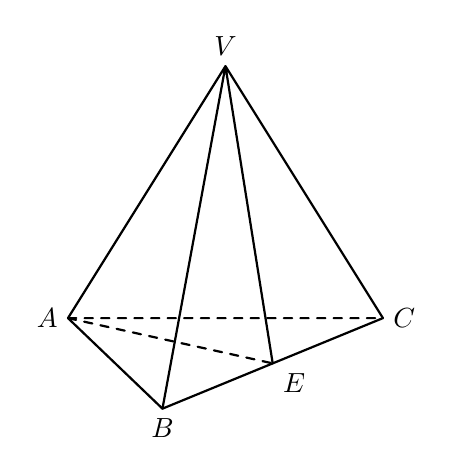
\begin{tikzpicture}[line cap=round,line join=round,thick]
  \coordinate (V) at (0,3.2);
  \coordinate (A) at (-2.0,0);
  \coordinate (B) at (-0.8,-1.15);
  \coordinate (C) at (2.0,0);
  \coordinate (E) at (0.6,-0.575);

  % Visible pyramid edges and the median in face VBC.
  \draw (V)--(A) (V)--(B) (V)--(C) (V)--(E);
  \draw (A)--(B)--(C);

  % Hidden rear base edge and the indicated segment AE.
  \draw[dashed] (A)--(C) (A)--(E);

  \node[above] at (V) {$V$};
  \node[left] at (A) {$A$};
  \node[below] at (B) {$B$};
  \node[right] at (C) {$C$};
  \node[below right] at (E) {$E$};
\end{tikzpicture}
\end{center}
\nopagebreak[4]
\Needspace{4\baselineskip}
\textbf{解析}

\Needspace{5\baselineskip}
设 $O$ 为等边底面 $ABC$ 的中心。$AE=\sqrt3$，且 $O\in AE$、$VO\perp$ 底面，故 $VO$ 也是 $V$ 到 $AE$ 的距离。面积条件给出

\nopagebreak[4]
\[\frac12 AE\cdot VO=\frac14,\qquad VO=\frac1{2\sqrt3}.\]

\Needspace{5\baselineskip}
等边三角形边长为 $2$，故 $AO=2/\sqrt3$。侧棱 $VA$ 与底面所成角为 $\angle VAO$，于是

\nopagebreak[4]
\[\tan\angle VAO=\frac{VO}{AO}=\frac14.\]

\gkanswer{答案：$\arctan\dfrac14$}

\end{answer}
\begin{answer}
\gksolhead{7}{}

\textbf{题目}：

在数列 $\{a_n\}$ 中，$a_1=3$，且对任意大于 $1$ 的正整数 $n$，点 $(\sqrt{a_n},\sqrt{a_{n-1}})$ 在直线 $x-y-\sqrt{3}=0$ 上，则 $\displaystyle\lim_{n\to\infty}\dfrac{a_n}{(n+1)^2}=\underline{\qquad}$。

\Needspace{4\baselineskip}
\textbf{解析}

\Needspace{5\baselineskip}
点 $(\sqrt{a_n},\sqrt{a_{n-1}})$ 在 $x-y-\sqrt3=0$ 上，故

\nopagebreak[4]
\[\sqrt{a_n}-\sqrt{a_{n-1}}=\sqrt3.\]

\Needspace{5\baselineskip}
结合 $\sqrt{a_1}=\sqrt3$，归纳得 $\sqrt{a_n}=n\sqrt3$，即 $a_n=3n^2$。因此

\nopagebreak[4]
\[\lim_{n\to\infty}\frac{a_n}{(n+1)^2}=3.\]

\gkanswer{答案：$3$}

\end{answer}
\begin{answer}
\gksolhead{8}{}

\textbf{题目}：

根据下列 $5$ 个图形及相应点的个数的变化规律，试猜测第 $n$ 个图形中有 $\underline{\qquad}$ 个点。
\nopagebreak[4]
\begin{center}% Q8：逐点复现原页的五个空心圆点阵，不据此添加题目未给的几何条件。
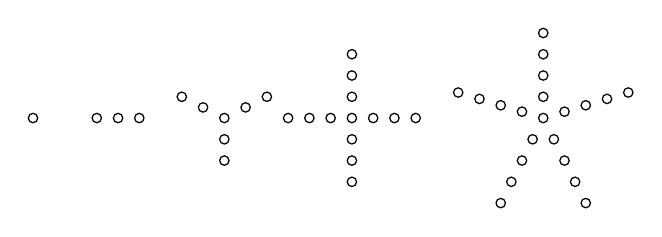
\begin{tikzpicture}[x=0.27cm,y=0.27cm,line width=0.45pt]
  \foreach \x/\y in {
    0/0,
    3/0,4/0,5/0,
    7/1,8/0.5,9/0,10/0.5,11/1,9/-1,9/-2,
    15/-3,15/-2,15/-1,15/0,15/1,15/2,15/3,
    12/0,13/0,14/0,16/0,17/0,18/0,
    24/4,24/3,24/2,24/1,
    20/1.2,21/0.9,22/0.6,23/0.3,24/0,25/0.3,26/0.6,27/0.9,28/1.2,
    23.5/-1,24.5/-1,23/-2,25/-2,22.5/-3,25.5/-3,22/-4,26/-4
  } {
    \draw[fill=white] (\x,\y) circle[radius=1.7pt];
  }
\end{tikzpicture}
\end{center}
\nopagebreak[4]
\Needspace{4\baselineskip}
\textbf{解析}

\Needspace{5\baselineskip}
图中点数依次为 $1,3,7,13,21$，相邻差为 $2,4,6,8$。第 $n$ 项为

\nopagebreak[4]
\[1+\sum_{k=1}^{n-1}2k=1+n(n-1)=n^2-n+1.\]

\gkanswer{答案：$n^2-n+1$}

\end{answer}
\begin{answer}
\gksolhead{9}{}

\textbf{题目}：

一次二期课改经验交流会打算交流试点学校的论文 $5$ 篇和非试点学校的论文 $3$ 篇。若任意排列交流次序，则最先和最后交流的论文都为试点学校的概率是 $\underline{\qquad}$。（结果用分数表示。）

\Needspace{4\baselineskip}
\textbf{解析}

\Needspace{5\baselineskip}
将首尾两个位置依次抽取，均为试点学校论文的概率为

\nopagebreak[4]
\[\frac58\cdot\frac47=\frac5{14}.\]

\gkanswer{答案：$\dfrac5{14}$}

\end{answer}
\begin{answer}
\gksolhead{10}{}

\textbf{题目}：

若平移椭圆 $4(x+3)^2+9y^2=36$，使平移后的椭圆中心在第一象限，且它与 $x$ 轴、$y$ 轴分别只有一个交点，则平移后的椭圆方程是 $\underline{\qquad}$。

\Needspace{4\baselineskip}
\textbf{解析}

\Needspace{5\baselineskip}
原椭圆半轴长分别为 $3$、$2$。平移后中心 $(h,k)$ 在第一象限；椭圆与 $y$ 轴仅有一个交点，说明其与 $y$ 轴相切，故 $h=3$；与 $x$ 轴仅有一个交点，故 $k=2$。于是

\nopagebreak[4]
\[\frac{(x-3)^2}{9}+\frac{(y-2)^2}{4}=1.\]

\gkanswer{答案：$4(x-3)^2+9(y-2)^2=36$}

\end{answer}
\begin{answer}
\gksolhead{11}{}

\textbf{题目}：

如图，在由二项式系数所构成的杨辉三角形中，第 $\underline{\qquad}$ 行中从左至右第 $14$ 与第 $15$ 个数的比为 $2:3$。
\nopagebreak[4]
\begin{center}% Q11：忠实排出原页可见的杨辉三角前六行及行号。
\begin{tikzpicture}[x=0.78cm,y=0.62cm]
  \foreach \r in {0,...,5} {
    \node[anchor=east] at (-3.2,-\r) {第 \r 行};
  }
  \node at (0,0) {1};
  \node at (-0.5,-1) {1}; \node at (0.5,-1) {1};
  \node at (-1,-2) {1}; \node at (0,-2) {2}; \node at (1,-2) {1};
  \node at (-1.5,-3) {1}; \node at (-0.5,-3) {3};
  \node at (0.5,-3) {3}; \node at (1.5,-3) {1};
  \node at (-2,-4) {1}; \node at (-1,-4) {4}; \node at (0,-4) {6};
  \node at (1,-4) {4}; \node at (2,-4) {1};
  \node at (-2.5,-5) {1}; \node at (-1.5,-5) {5}; \node at (-0.5,-5) {10};
  \node at (0.5,-5) {10}; \node at (1.5,-5) {5}; \node at (2.5,-5) {1};
  \node[anchor=east] at (-2.5,-6) {$\cdots\cdots$};
  \node at (0,-6) {$\cdots\cdots$};
\end{tikzpicture}
\end{center}
\nopagebreak[4]
\Needspace{4\baselineskip}
\textbf{解析}

\Needspace{5\baselineskip}
按第 $n$ 行对应二项式系数 $\binom n0,\ldots,\binom nn$（首行为第 $0$ 行），从左至右第 $14$、$15$ 个数之比为

\nopagebreak[4]
\[\frac{\binom n{13}}{\binom n{14}}=\frac{14}{n-13}=\frac23.\]

解得 $n=34$。

\gkanswer{答案：第 $34$ 行（以第 0 行为首行）}

\end{answer}
\begin{answer}
\gksolhead{12}{}

\textbf{题目}：

在等差数列 $\{a_n\}$ 中，当 $a_r=a_s$（$r\ne s$）时，$\{a_n\}$ 必定是常数数列。然而在等比数列 $\{a_n\}$ 中，对某些正整数 $r,s$（$r\ne s$），当 $a_r=a_s$ 时，非常数数列 $\{a_n\}$ 的一个例子是 $\underline{\qquad}$。

\Needspace{4\baselineskip}
\textbf{解析}

取公比 $q=-1$、首項 $a_1=1$，则 $a_n=(-1)^{n-1}$。这是非恒定等比数列，且 $a_1=a_3=1$，符合要求。

\gkanswer{答案：例如 $a_n=(-1)^{n-1}$}

\end{answer}
\begin{answer}
\gksolhead{13}{}

\textbf{题目}：

下列函数中，周期为 $1$ 的奇函数是\mbox{（　　）}。

（A）$y=1-2\sin^2\pi x$　　（B）$y=\sin\left(2\pi x+\dfrac{\pi}{3}\right)$\\
（C）$y=\tan\dfrac{\pi}{2}x$　　（D）$y=\sin\pi x\cos\pi x$

\Needspace{4\baselineskip}
\textbf{解析}

\Needspace{5\baselineskip}
(A) $1-2\sin^2\pi x=\cos2\pi x$ 为偶函数；(B) 虽周期为 $1$，但相位平移后不是奇函数；(C) $\tan(\pi x/2)$ 的周期为 $2$。而

\nopagebreak[4]
\[\sin\pi x\cos\pi x=\frac12\sin2\pi x\]

为奇函数，周期为 $1$。

\gkanswer{答案：D}

\end{answer}
\begin{answer}
\gksolhead{14}{}

\textbf{题目}：

若非空集合 $M\subseteq N$，则“$a\in M$ 或 $a\in N$”是“$a\in M\cap N$”的\mbox{（　　）}。

（A）充分非必要条件　　（B）必要非充分条件\\
（C）充要条件　　（D）既非充分又非必要条件

\Needspace{4\baselineskip}
\textbf{解析}

因 $M\subseteq N$，命题“$a\in M$ 或 $a\in N$”等价于 $a\in N$，而 $a\in M\cap N$ 等价于 $a\in M$。若原题意为真包含 $M\subsetneq N$，后者能推出前者而反向不成立，选（B）；但原卷印的是允许相等的 $M\subseteq N$。若 $M=N$，两命题等价，应选（C）。因此在没有同版勘误或其他可靠材料明确“真包含”之前，原题条件不足以唯一确定选项，本答案保留待核，不擅自指定 B 或 C。

\textbf{条件结论：}$M\subsetneq N$ 时为（B）；$M=N$ 时为（C）。原题答案待核。

\gkanswer{答案：U/PENDING；答案待核；若 $M\subsetneq N$ 则 B；若 $M=N$ 则 C。}

\end{answer}
\begin{answer}
\gksolhead{15}{}

\textbf{题目}：

在 $\triangle ABC$ 中，有命题：① $\overrightarrow{AB}-\overrightarrow{AC}=\overrightarrow{BC}$；② $\overrightarrow{AB}+\overrightarrow{BC}+\overrightarrow{CA}=\vec{0}$；③ 若 $(\overrightarrow{AB}+\overrightarrow{AC})\cdot(\overrightarrow{AB}-\overrightarrow{AC})=0$，则 $\triangle ABC$ 为等腰三角形；④ 若 $\overrightarrow{AC}\cdot\overrightarrow{AB}>0$，则 $\triangle ABC$ 为锐角三角形。上述命题正确的是\mbox{（　　）}。

（A）①②　　（B）①④　　（C）②③　　（D）②③④

\Needspace{4\baselineskip}
\textbf{解析}

① $\overrightarrow{AB}-\overrightarrow{AC}=\overrightarrow{CB}$，不是 $\overrightarrow{BC}$；② 为三角形的闭合向量关系，成立；③ 左式等于 $|AB|^2-|AC|^2$，为 $0$ 时 $AB=AC$，成立；④ 只说明 $\angle A$ 为锐角，不能推出其余两角均锐角。因此仅②③正确。

\gkanswer{答案：C}

\end{answer}
\begin{answer}
\gksolhead{16}{}

\textbf{题目}：

若 $p=a+\dfrac{1}{a}+2$（$a>0$），$q=\arccos t$（$-1\le t\le1$），则下列不等式恒成立的是\mbox{（　　）}。

（A）$p\ge\pi>q$　　（B）$p>q\ge0$　　（C）$4>p\ge q$　　（D）$p\ge q>0$

\Needspace{4\baselineskip}
\textbf{解析}

由 $a>0$ 及均值不等式，$p=a+1/a+2\ge4$；又 $q=\arccos t\in[0,\pi]$。因此 $p>q\ge0$。

\gkanswer{答案：B}

\end{answer}
\begin{answer}
\gksolhead{17}{}

\textbf{题目}：

在直角坐标系 $xOy$ 中，已知点 $P(2\cos x+1,\,2\cos 2x+2)$ 和点 $Q(\cos x,-1)$，其中 $x\in[0,\pi]$。若向量 $\overrightarrow{OP}$ 与 $\overrightarrow{OQ}$ 垂直，求 $x$ 的值。

\Needspace{4\baselineskip}
\textbf{解析}

\Needspace{5\baselineskip}
令 $c=\cos x$，则 $\cos2x=2c^2-1$，从而 $P=(2c+1,4c^2)$、$Q=(c,-1)$。垂直条件为

\nopagebreak[4]
\[\overrightarrow{OP}\cdot\overrightarrow{OQ}=(2c+1)c-4c^2=c(1-2c)=0.\]

故 $c=0$ 或 $c=1/2$。在 $x\in[0,\pi]$ 内，分别得 $x=\pi/2$、$x=\pi/3$。

\gkanswer{答案：$x=\dfrac\pi3$ 或 $x=\dfrac\pi2$}

\end{answer}
\begin{answer}
\gksolhead{18}{}

\textbf{题目}：

已知实数 $p$ 满足不等式 $\dfrac{2x+1}{x+2}<0$，试判断方程 $z^2-2z+5-p^2=0$ 有无实根，并给出证明。

\begin{gktip}
\textbf{原文疑点}：原件印作“实数 $p$ 满足不等式”，但该不等式使用变量 $x$；本稿按原件保留，未将 $x$ 擅改为 $p$。该疑点影响题意解释，待取得可追溯的同版答案/勘误或其他直接来源后复核。
\end{gktip}

\Needspace{4\baselineskip}
\textbf{解析}

\Needspace{5\baselineskip}
原文写作“实数 $p$ 满足 $\dfrac{2x+1}{x+2}<0$”，其中条件中的变量是 $x$，并未约束 $p$。按字面，该不等式的解集为 $-2<x<-1/2$，但不影响 $p$ 的取值。方程关于 $z$ 的判别式为

\nopagebreak[4]
\[\Delta=(-2)^2-4(5-p^2)=4(p^2-4).\]

所以按当前字面，$|p|\ge2$ 时有实根，$|p|<2$ 时无实根；题目不能据所给条件给出唯一的“有/无实根”结论。若经可靠原件证据确认条件本应为 $\dfrac{2p+1}{p+2}<0$，则 $-2<p<-1/2$，故 $|p|<2$，方程无实根。当前不选择其中一个解释冒充确定题意。

\gkanswer{答案：原文中约束不等式含 $x$ 而非 $p$，因此不能确定 $p$。按字面，方程有实根当且仅当 $|p|\ge2$；若原意为 $\dfrac{2p+1}{p+2}<0$，则 $-2<p< -\dfrac12$，方程无实根。此结论待原题变量疑点裁定。}

\end{answer}
\begin{answer}
\gksolhead{19}{}

\textbf{题目}：

某市 $2003$ 年共有 $1$ 万辆燃油型公交车。有关部门计划于 $2004$ 年投入 $128$ 辆电力型公交车，随后电力型公交车每年的投入比上一年增加 $50\%$。试问：

（1） 该市在 $2010$ 年应该投入多少辆电力型公交车？

（2） 到哪一年底，电力型公交车的数量开始超过该市公交车总量的 $\dfrac{1}{3}$？

\Needspace{4\baselineskip}
\textbf{解析}

\gksubpart{(1)}

\Needspace{5\baselineskip}
设 $a_1=128$ 为 2004 年投入量，公比 $q=3/2$。2010 年为第 $7$ 项，故

\nopagebreak[4]
\[a_7=128\left(\frac32\right)^6=1458.\]

\gksubpart{(2)}

到某年年底累计投入的电力公交车数为 $S_m=128((3/2)^m-1)/(1/2)=256((3/2)^m-1)$，其中 $m$ 是从 2004 年起计的年数。电力公交超过总车数 $1/3$ 等价于 $E>(10000+E)/3$，即 $E>5000$。至 2010 年底累计 $S_7=4118<5000$；至 2011 年底 $S_8=6305>5000$。故从 2011 年底开始超过该比例。

\gkanswer{答案（1）：$1458$ 辆}

\gkanswer{答案（2）：2011 年底}

\end{answer}
\begin{answer}
\gksolhead{20}{}

\textbf{题目}：

如图，点 $P$ 为斜三棱柱 $ABC-A_1B_1C_1$ 的侧棱 $BB_1$ 上一点，$PM\perp BB_1$ 交 $AA_1$ 于点 $M$，$PN\perp BB_1$ 交 $CC_1$ 于点 $N$。

（1） 求证：$CC_1\perp MN$；

（2） 在任意 $\triangle DEF$ 中有余弦定理：$DE^2=DF^2+EF^2-2DF\cdot EF\cos\angle DFE$。拓展到空间，类比三角形的余弦定理，写出斜三棱柱的三个侧面面积与其中两个侧面所成的二面角之间的关系式，并予以证明。
\nopagebreak[4]
\begin{center}% Q20：按原图复现斜三棱柱的顶点、可见/隐藏棱及 P,M,N 辅助线。
% 投影为示意布局，不表达未给出的长度或角度。
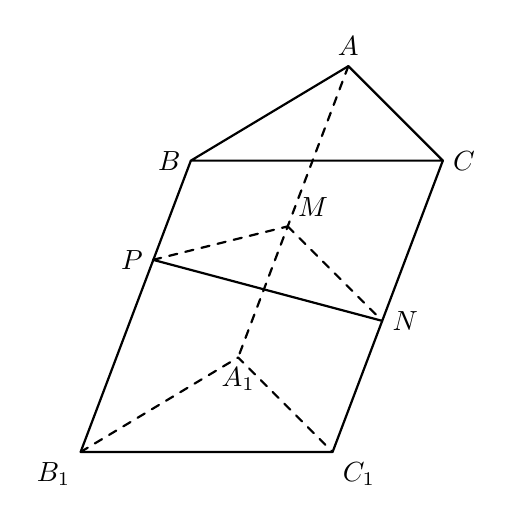
\begin{tikzpicture}[line cap=round,line join=round,thick]
  \coordinate (A)  at (2.0,4.0);
  \coordinate (B)  at (0.0,2.8);
  \coordinate (C)  at (3.2,2.8);
  \coordinate (A1) at (0.6,0.3);
  \coordinate (B1) at (-1.4,-0.9);
  \coordinate (C1) at (1.8,-0.9);
  \coordinate (P)  at (-0.48,1.54);
  \coordinate (M)  at (1.23,1.965);
  \coordinate (N)  at (2.43,0.765);

  % Upper face and visible prism edges.
  \draw (A)--(B)--(C)--(A);
  \draw (B)--(B1) (C)--(C1) (B1)--(C1);

  % Hidden back edge and rear triangular face.
  \draw[dashed] (A)--(A1) (B1)--(A1)--(C1);

  % Auxiliary construction shown in the original.
  \draw[dashed] (P)--(M) (M)--(N);
  \draw (P)--(N);

  \node[above] at (A) {$A$};
  \node[left] at (B) {$B$};
  \node[right] at (C) {$C$};
  \node[below] at (A1) {$A_1$};
  \node[below left] at (B1) {$B_1$};
  \node[below right] at (C1) {$C_1$};
  \node[left] at (P) {$P$};
  \node[above right] at (M) {$M$};
  \node[right] at (N) {$N$};
\end{tikzpicture}
\end{center}
\nopagebreak[4]
\Needspace{4\baselineskip}
\textbf{解析}

\gksubpart{(1)}

棱柱侧棱 $AA_1,BB_1,CC_1$ 互相平行。由 $PM\perp BB_1$、$PN\perp BB_1$，且 $M,N,P$ 共面于垂直于侧棱的截面平面，故该平面内的 $MN\perp BB_1$，从而 $MN\perp CC_1$。

\gksubpart{(2)}

\Needspace{5\baselineskip}
记 $S_{AB},S_{AC},S_{BC}$ 分别为平行四边形侧面 $ABB_1A_1,ACC_1A_1,BCC_1B_1$ 的面积；令 $\theta$ 为平面 $BCC_1B_1$ 与平面 $ACC_1A_1$ 沿 $CC_1$ 所成的二面角。因为 $PM,PN,MN$ 都在垂直于侧棱的截面平面 $PMN$ 内，$\angle MNP=\theta$，且

\nopagebreak[4]
\[S_{AB}=PM\cdot BB_1=PM\cdot CC_1,\quad S_{BC}=PN\cdot CC_1,\quad S_{AC}=MN\cdot CC_1.\]

\Needspace{5\baselineskip}
在 $\triangle PMN$ 中用余弦定理，并将等式两边乘以 $CC_1^2$，得

\nopagebreak[4]
\[S_{AB}^2=S_{BC}^2+S_{AC}^2-2S_{BC}S_{AC}\cos\theta.\]

\gkanswer{答案（1）：$CC_1\perp MN$}

\gkanswer{答案（2）：$S_{AB}^2=S_{BC}^2+S_{AC}^2-2S_{BC}S_{AC}\cos\theta$}

\end{answer}
\begin{answer}
\gksolhead{21}{}

\textbf{题目}：

已知函数 $f(x)=|x-a|$，$g(x)=x^2+2ax+1$（$a$ 为正常数），且函数 $f(x)$ 与 $g(x)$ 的图象在 $y$ 轴上的截距相等。

（1） 求 $a$ 的值；

（2） 求函数 $f(x)+g(x)$ 的单调递增区间；

（3） 若 $n$ 为正整数，证明：$10^{f(n)}\cdot\left(\dfrac{4}{5}\right)^{g(n)}<4$。

\Needspace{4\baselineskip}
\textbf{解析}

\gksubpart{(1)}

两图象在 $y$ 轴上的截距分别为 $a$、$1$，故 $a=1$。

\gksubpart{(2)}

\Needspace{5\baselineskip}
此时

\nopagebreak[4]
\[f(x)+g(x)=\begin{cases}x^2+x+2,&x<1,\\x^2+3x,&x\ge1.\end{cases}\]

第一段导数为 $2x+1$，在 $x\ge-1/2$ 时非负；第二段导数为 $2x+3>0$。两段在 $x=1$ 连续相接，且该处右侧仍递增，故递增区间为 $[-1/2,+\infty)$。

\gksubpart{(3)}

\Needspace{5\baselineskip}
对正整数 $n$，$f(n)=n-1$、$g(n)=(n+1)^2$。令

\nopagebreak[4]
\[u_n=10^{n-1}\left(\frac45\right)^{(n+1)^2}.\]

\Needspace{5\baselineskip}
有

\nopagebreak[4]
\[\frac{u_{n+1}}{u_n}=10\left(\frac45\right)^{2n+3}.\]

该比值随 $n$ 递减；在 $n=3$ 时仍大于 $1$，在 $n=4$ 时小于 $1$。故 $(u_n)$ 的最大值为 $u_4=1000(4/5)^{25}<4$（等价于 $250\cdot4^{25}<5^{25}$，整数比较成立），从而对所有正整数 $n$ 均有 $u_n<4$。

\gkanswer{答案（1）：$a=1$}

\gkanswer{答案（2）：$[-\dfrac12,+\infty)$}

\gkanswer{答案（3）：命题成立。}

\end{answer}
\begin{answer}
\gksolhead{22}{}

\textbf{题目}：

已知倾斜角为 $45^\circ$ 的直线 $l$ 过点 $A(1,-2)$ 和点 $B$，$B$ 在第一象限，$|AB|=3\sqrt{2}$。

（1） 求点 $B$ 的坐标；

（2） 若直线 $l$ 与双曲线 $C:\dfrac{x^2}{a^2}-y^2=1$（$a>0$）相交于 $E$、$F$ 两点，且线段 $EF$ 的中点坐标为 $(4,1)$，求 $a$ 的值；

（3） 对于平面上任一点 $P$，当点 $Q$ 在线段 $AB$ 上运动时，称 $|PQ|$ 的最小值为点 $P$ 与线段 $AB$ 的距离。已知点 $P$ 在 $x$ 轴上运动，写出点 $P(t,0)$ 到线段 $AB$ 的距离 $h$ 关于 $t$ 的函数关系式。

\Needspace{4\baselineskip}
\textbf{解析}

\gksubpart{(1)}

直线方向角为 $45^\circ$，方向向量可取 $(1,1)$。由 $|AB|=3\sqrt2$，从 $A(1,-2)$ 沿此方向前进 $3$ 倍得到第一象限点 $B=(4,1)$（反向得到 $(-2,-5)$，不在第一象限）。因此 $l:y=x-3$。

\gksubpart{(2)}

\Needspace{5\baselineskip}
联立双曲线与直线：

\nopagebreak[4]
\[\frac{x^2}{a^2}-(x-3)^2=1.\]

交点横坐标为关于 $x$ 的二次方程两根，和为中点横坐标的两倍，即 $8$。比较二次项系数 $1/a^2-1$ 与一次项系数 $6$，根和为 $-6/(1/a^2-1)=8$，故 $1/a^2=1/4$，即 $a=2$。

\gksubpart{(3)}

\Needspace{5\baselineskip}
令 $P=(t,0)$，线段方向向量为 $d=(3,3)$。垂足参数

\nopagebreak[4]
\[s=\frac{(P-A)\cdot d}{|d|^2}=\frac{t+1}{6}.\]

当 $-1\le t\le5$ 时垂足落在线段上，到直线 $y=x-3$ 的距离是 $|t-3|/\sqrt2$。当 $t<-1$ 时最近点为端点 $A$，距离为 $\sqrt{(t-1)^2+4}$；当 $t>5$ 时最近点为端点 $B$，距离为 $\sqrt{(t-4)^2+1}$。所求分段函数见答案。

\gkanswer{答案（1）：$B=(4,1)$}

\gkanswer{答案（2）：$a=2$}

\gkanswer{答案（3）：$h(t)=\begin{cases}\sqrt{(t-1)^2+4},&t<-1,\\\dfrac{|t-3|}{\sqrt2},&-1\le t\le5,\\\sqrt{(t-4)^2+1},&t>5.\end{cases}$}

\end{answer}